\documentclass[12pt]{article}

\usepackage[cm]{fullpage}
\usepackage{graphicx}
\usepackage{url}
\pagenumbering{gobble}

\linespread{1.00}

\usepackage{titlesec} % Allows customization of titles

\setlength\parindent{24pt}

\usepackage[
  top    = 1.50cm,
  bottom = 1.50cm,
  left   = 1.50cm,
  right  = 1.50cm]{geometry}

\usepackage{setspace}

\title{\vspace{-25mm}\fontsize{16pt}{10pt}\selectfont\textbf{DCP: Fast Recursive Copy}} % Article title

\author{
  \textsc{William Morriss} \\
  \textsc{Thomas Kim}
}
\date{}

\begin{document}

\maketitle % Insert title

\section{Overview}
An improved version of 'cp -r,' dcp, was implemented.
This version takes advantage of Linux's asynchronous IO interfaces to create
opportunities for parallelism, and minimizes the time spent blocking on disk
IO by leveraging fallocate and readahead. In order to ensure reads
are more likely to result in hits in the buffer cache when memory is scarce, POSIX
fadvise is used. To ensure optimal layout of files for writing, POSIX
fallocate is used. The main goal of dcp is to fully saturate disk IO
at all times in order to have a fast, portable solution which supports
any POSIX compliant filesystem interface. \\

GNU coreutils has rejected \cite{rejected} a number of feature requests and one of them was
``cp --parallel'', which would read and write from different file offsets in
parallel \cite{cppara}. This feature was rejected on the suggestion of using multiple dd
processes instead and its github project \cite{pcopy} is incomplete and
inactive. Splitting larger files may in fact improve performance but this project
did not explore it.

\section{Implementation}

\subsection{MPSCQ}
The implementation uses a multi-producer, single-consumer queue (MPSCQ) to manage its
work queue. The producers are the asynchronous directory read operations and
the consumer is the main loop, which begins work and limits in-progress task
count. \\

The MPSCQ is implemented with a linked list and atomic compare exchange instructions.
The consumer has a pointer to the next node to be freed. Its next data to read
is in the next node, so an empty list has one node. This way, the consumer frees
one node per read. Each linked list node is annotated with a count and each
node's count is one more than the previous. A producer creates the next node in
its entirety based on its understanding of the end of the queue and then
compare exchanges the address of that node into the node's next pointer,
expecting NULL. To assist future threads in finding the end, it does compare
exchange on the linked list's tail in a loop until either its proposed node is
the tail or a node of greater count is the tail.
The MPSCQ is thus lock free but not wait free and would be interrupt-reentrant
safe as well (discussion below) if it did not call glibc malloc. \\
% TODO show pseudocode

\subsection{Multithreading}
The implementation uses the POSIX asynchronous i/o ~\cite{aio}. Job completion was initially
received with a signal (SIGEV\_SIGNAL) and the file work was entirely signal-driven
but interrupts were happening at antagonistic times within and without interrupt
handlers. In particular, glibc lazily protects aio with a reentrant mutex, so an
interrupt handler within an interrupt handler would violate its interrupted handler's
critical section. Iniitially this was fixed by making a MPSCQ for aio operations to schedule
so that they were scheduled by the main loop and not by handlers but this deadlocked with low
probability because glibc malloc, required by the MPSCQ, is protected by a spinlock and
would be interrupted inside its critical section and that interrupt would not be
able to acquire the lock from itself. Moving off of signals and onto threads (SIGEV\_THREAD)
vastly simplified the implementation and got around all of those pesky single-threaded
concurrency issues. \\

\subsection{Readahead and buffer size}
POSIX fadvise is used to ensure that pages will be available
in the buffer cache when read~\cite{fadvise}, and that pages will be evicted from
the cache as soon as possible. All reads in dcp are
sequential, so FADV\_SEQUENTIAL is used. \\

Additionally, readahead is used to provide hints to the kernel
regarding the number of bytes which should be read into the buffer cache.
Currently, dcp uses a fixed-size buffer of 0x80000 bytes for reads.
As part of future work, a buffer which adaptively resizes itself based on system
load and IO speed is proposed. However, adaptively resizing the buffer introduces
some overhead and it is difficult to tune the size of the buffer for performance gains
in all workloads and across all systems. \\%TODO do we need this paragraph?

\subsection{Fallocate}
POSIX fallocate is used to allow the destination filesystem to
allocate blocks in an efficient way ~\cite{fallocate}. The copying program knows
the source file size and supplies it to the operating system.
The use of fallocate is fairly straightforward and measurably
increases write speeds on target ext4 filesystems, as demonstrated
by some of the following benchmarks. \\

\section {Test platforms}
\textbf{Test Platform 1}\\
\begin{tabular}{|l|r|r|}
  \hline
  Component & Specification                   & Interface \\
  CPU       & Intel i7-4770k @ 3.50GHz        &           \\
  RAM       & 8 GB @ 1333 Mhz                 &           \\
  OS        & Linux 3.13.0                    &           \\
  HDD A     &         1TB @ 7200rpm           & SATA II   \\
  HDD B     &                 2TB @ 5600rpm   & SATA II   \\
  SSD A     &         250GB                   & SATA II   \\
  External A& 3TB @ 5400rpm                   & USB 3.0   \\
  \hline
\end{tabular}\\\\
\textbf{Test Platform 2}\\
\begin{tabular}{|l|r|r|}
  \hline
  Component & Specification                   & Interface \\
  CPU       & Intel i7-2670QM @ 2.20GHz       &           \\
  RAM       & 8 GB @ 1333 MHz                 &           \\
  OS        & Linux 3.17.4-1                  &           \\
  HDD       & 1TB @ 5400rpm                   & SATA II 3.0Gb/s  \\
  \hline
\end{tabular}
\section{Benchmarking methodology}
Dcp was tested on consumer-grade personal computers using 3 different types
of drive: solid state drive, traditional disk-based hard drive, and
an external USB3.0 disk based hard drive. With the exception of the external
hard drive, which is formatted in NTFS, the disks are formatted in ext4.
The combinations of stable storage media tested include:\\
\begin{tabular}{|l|l|l|}
  \hline
  source  & destination & graph label \\
  \hline
  SSD A   & SSD A       & ssd - self  \\
  SSD A   & HDD A       & ssd - hdd   \\
  SSD A   & External A  & ssd - ext   \\
  HDD A   & SSD A       & hdd - ssd   \\
  HDD A   & HDD B       & hdd - hdd   \\
  HDD A   & External A  & hdd - ext   \\
  External A & SSD A    & ext - ssd   \\
  External A & HDD A    & ext - hdd   \\
  \hline
\end{tabular} \\\\

\noindent
These drive configurations were tested using test platform 1.

In addition to the tests done on different drive configurations,
dcp was benchmarked with certain optimizations disabled or modified, including
the number of threads, fadvise, and readahead. These tests were done on test platform 2.\\

In order to ensure that the benchmark files are not stored in the buffer cache
for subsequent executions of 'cp -r' or dcp, each benchmark was regenerated
before each execution using random data read from \texttt{/dev/urandom}.
Additionally, the resulting copied data from calling dcp
was compared to the generated data using 'diff -r' in order to
ensure that a full copy of the data was in fact executed.\\

An interesting problem which arose when testing these various combinations
was that HDD B and External A had aggressive power-saving mechanisms built into the
disk controller firmware. This caused inconsistent performance, which
manifested initially as a bimodal distribution of execution times. This
problem was remedied by running 'ls' on the root directory of the
drive immediately before running each test to ensure the disk was not in power-saving
mode.\\

Three main benchmarks were run on the data, named broad, fat, and deep.
These will be elaborated upon in the following section.\\

\section{Results}
The benchmarks were run 5 times each for dcp and 'cp -r,' and the execution
times were recorded. The sample mean and sample standard deviation were taken,
and a 2-sample 1-tailed unpaired t-test was executed to compare the execution
times for dcp and 'cp -r' for each disk configuration within a benchmark.\\

\subsection{Broad Benchmark}
Each file in the broad benchmark is 300kb (300000 bytes), and
the top level directory contains 7 files and 15 subdirectories. Each of the 15 subdirectories
contains 7 files and 15 subdirectories, which in turn contain 7 files.
The broad benchmark is similar to copying a  documents folder, as it is
relatively shallow but contains many subdirectories with files similar in size to
pdf documents. This benchmark was chosen to test dcp's ability to prioritize work
to keep IO saturated, as file reads blocking directory reads would severely bottleneck
the creation of new IO jobs and thus reduce saturation.\\
\noindent
The following graph shows the mean execution time across 5 trials of the broad benchmark across multiple disk configurations.
\vspace{5mm}

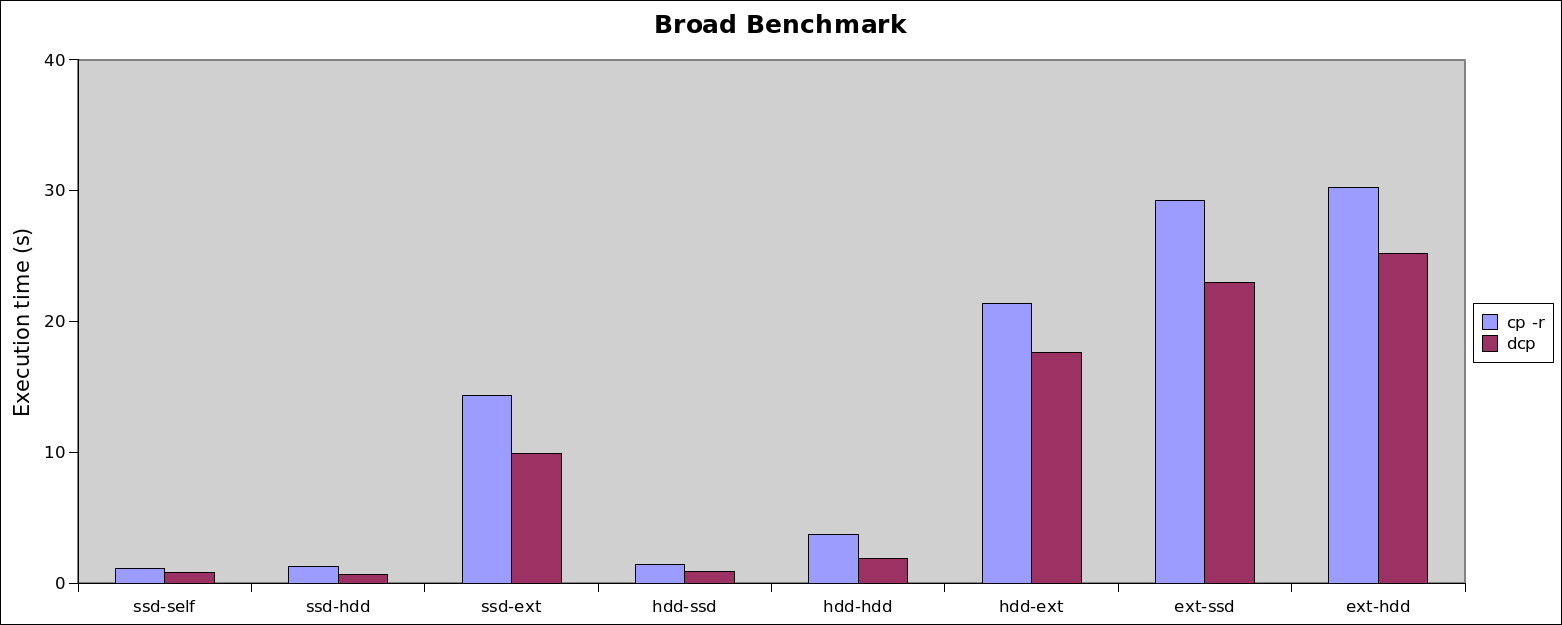
\includegraphics[width=500pt]{report/graphs/broad-manydisk.png}

\vspace{5mm}

The results show that dcp can gracefully handle workloads involving
similar numbers of directories and files, and prioritizes work
well to beat 'cp -r.' In all cases, $p < 0.005$, indicating that
the performance of dcp is statistically signficantly different from
that of 'cp -r,' and the graph clearly shows that dcp outperforms
'cp -r' on this benchmark. \\

The poor performance of the external
drive benchmarks is apparent here, and is a common theme throughout
the various tests run on the system. The external drive is not only
consistently slow, but also suffers from inconsistent throughput,
suffering from standard deviations from 1.5 for hdd-ext dcp
to 2.4 for ext-ssd 'cp -r' and dcp. This is likely due to the
extremely aggressive power-saving features of the external hard drive,
the relatively low rpm of the drive (5400) and the slow speed of the
USB interface. \\

Important to note here is that dcp outperformed 'cp -r' by a factor
of 1.9 on the hdd-hdd configuration and a factor of 1.7 on the
ssd-hdd configuration, which is important because these are common
usage patterns for many people. Backups are often done between disk drives
or from an SSD to a disk-based hard drive, and these cases are representative
of these situations. \\

The results of running the broad benchmark with certain optimizations turned
are displayed in the following graph.\\

\vspace{5mm}

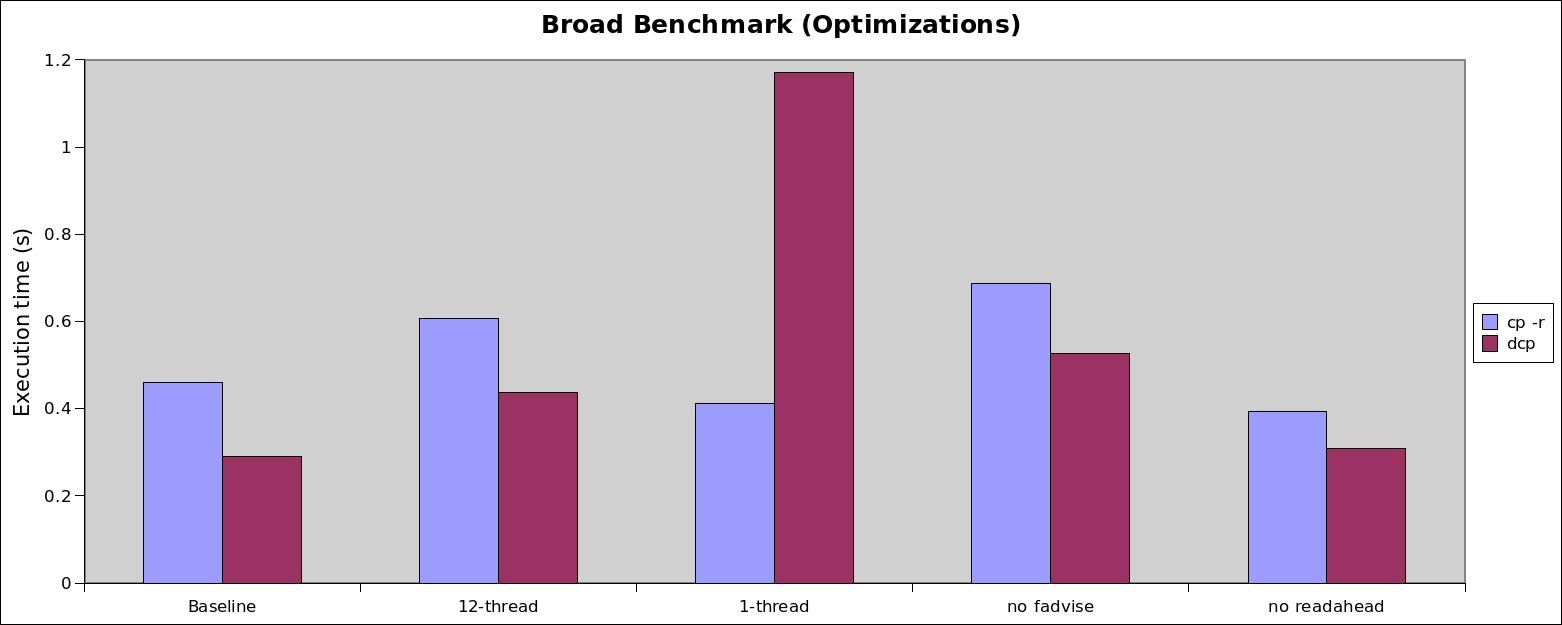
\includegraphics[width=500pt]{report/graphs/broad-optimizations.png}

\vspace{5mm}

Comparing the performance of unmodified dcp and dcp with certain
optimizations disabled, the statistically significant differences
from baseline include (using $\alpha = 0.05$) 1-thread ($p = 0.002$),
and no-fadvise ($p = 0.04$). This indicates that for the broad benchmark,
the more important optimizations include multithreading and fadvise. The
former is rather self-explanatory, and the latter makes sense as
broad uses somewhat large files which benefit from contiguous
block allocation on the target disk. \\

\subsection{Fat Benchmark}
Each file in the fat benchmark is 200kb (200000 bytes), and
the top level directory contains 3 files and 35 subdirectories. Each
of the 35 subdirectories contains 3 files and 35 subdirectories, which in turn contain 3 files.
The fat benchmark contains a large number of subdirectories and not many files per subdirectory.
This benchmark represents a sort of 'worst-case' for recursive copying, as files are small and numerous,
and directory trees have high branching factors with sparsely distributed files. This is an important
benchmark, as the performance of normal system copy utilities is often subpar for these operations,
so it is a prime target for optimization in dcp.
The following graph shows the mean execution time across 5 trials of the fat benchmark across multiple disk configurations. \\

\vspace{5mm}

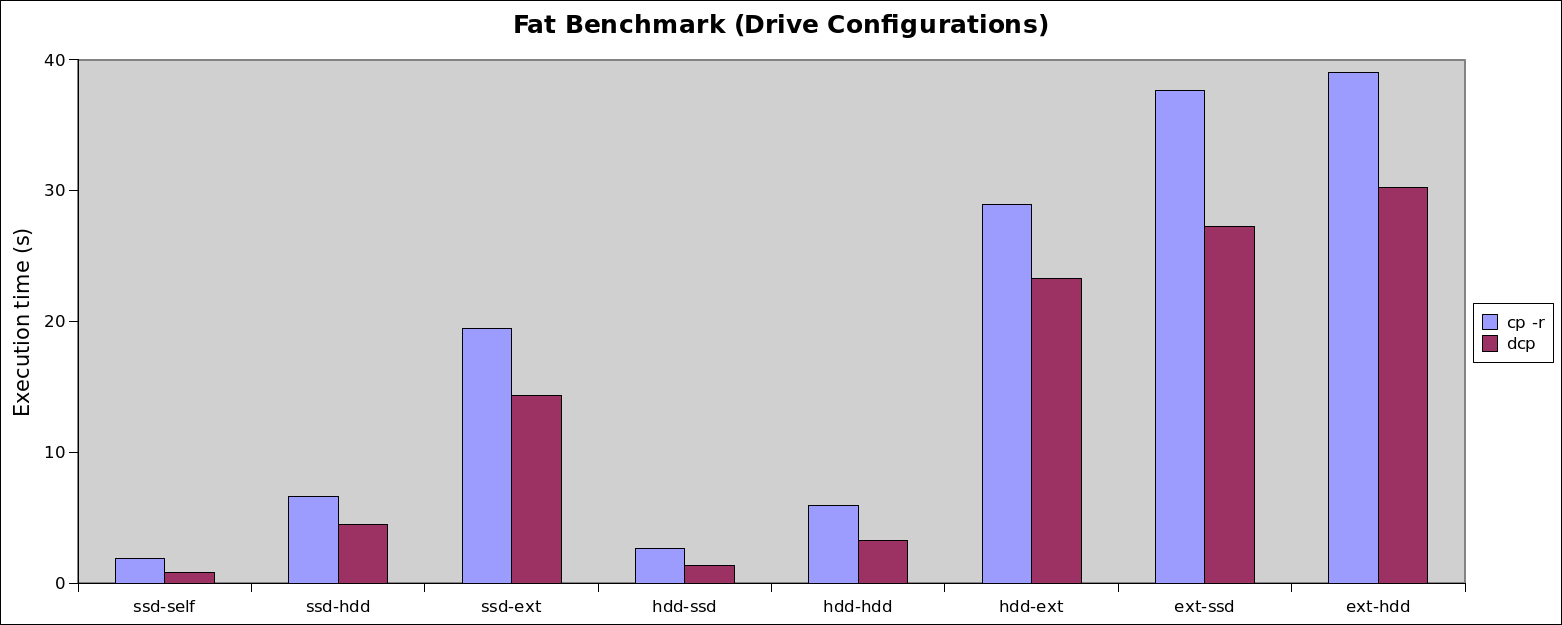
\includegraphics[width=500pt]{report/graphs/fat-manydisk.png}

\vspace{5mm}

Again, as with the broad benchmark results, the fat benchmark results confirm that
dcp consistently outperforms 'cp -r.' In all cases, the mean execution time for
dcp is statistically significantly lower than that of 'cp -r' ($p < 0.005$).
Again, in the important cases of ssd-hdd and hdd-hdd, dcp outperforms 'cp -r'
by a factor of 1.5 and 1.8 respectively. \\

The results of running the fast benchmark with certain optimizations turned
off are displayed in the following graph.\\

\vspace{5mm}

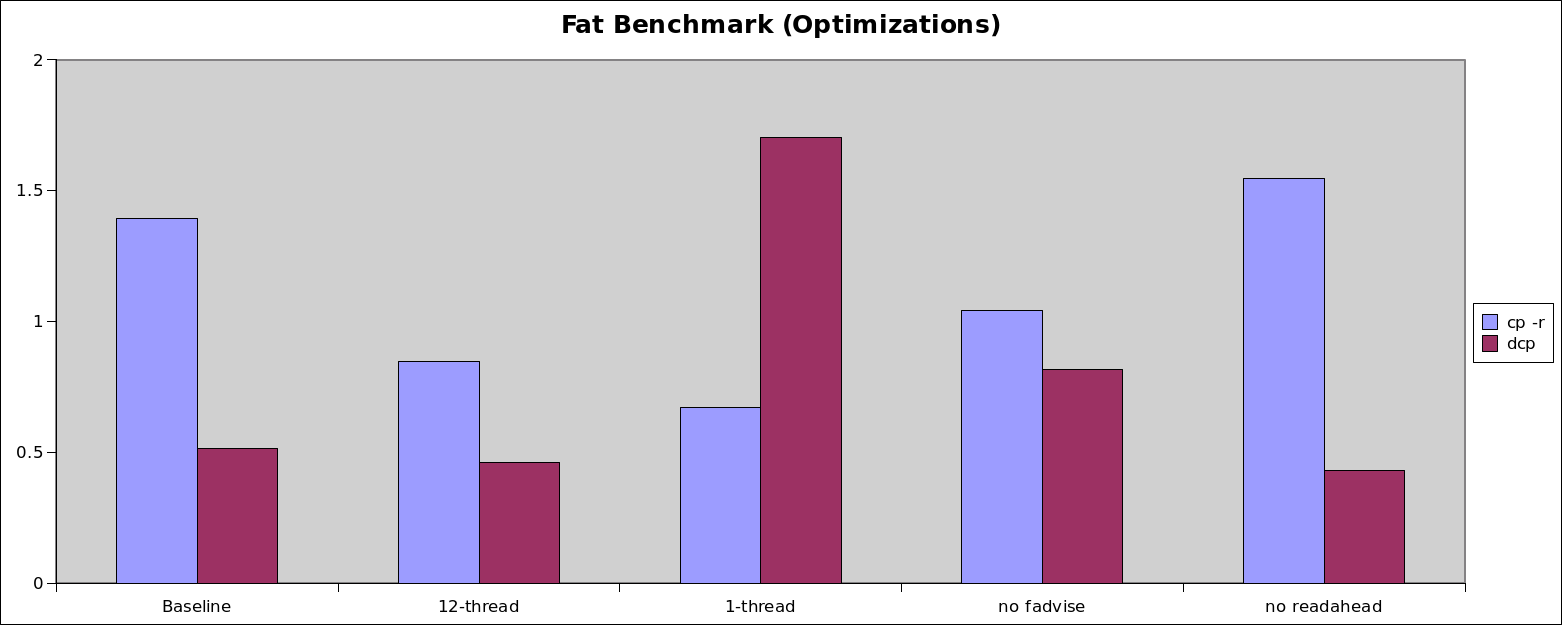
\includegraphics[width=500pt]{report/graphs/fat-optimizations.png}

\vspace{5mm}

The statistically significant performance decreases from baseline
include 1-thread ($p = 2 \times 10^{-7}$), 12-thread ($p = 0.04$), and no-readahead ($p = 0.009$).
Due to the larger number of smaller files and the high branching factor in the directory tree compared
to the broad benchmark, having 12 threads likely helped to saturate the IO speed since queueing/executing
these smaller jobs could possibly cause downtime with a smaller number of threads. This opens another question
of how to determine the number of simultaneous jobs being generated, as having too many threads generating jobs
could result in downtime due to threads contending for system resources, while having too few threads can
result in downtime if not enough jobs are generated to saturate IO. This angle is one which will be
explored in further research. \\

\subsection{Deep Benchmark}
Each file in the deep benchmark is 20mb (20000000 bytes), and
the top level directory contains 1 file and 1 subdirectory. There
are 6 nested subdirectories in this benchmark.
The deep benchmark is purposely small in order to ensure that dcp prioritizes
directories over files in such a way that it avoids blocking as much as possible.
If dcp were to prioritize reading and writing files over directories, it would end up
blocking on all 6 subdirectories and thus would lose to 'cp -r.' This is demonstrated
when evaluating the performance of dcp with certain optimizations removed. \\

\noindent
The following graph shows the mean execution time across 5 trials of the deep benchmark across multiple disk configurations. \\

\vspace{5mm}

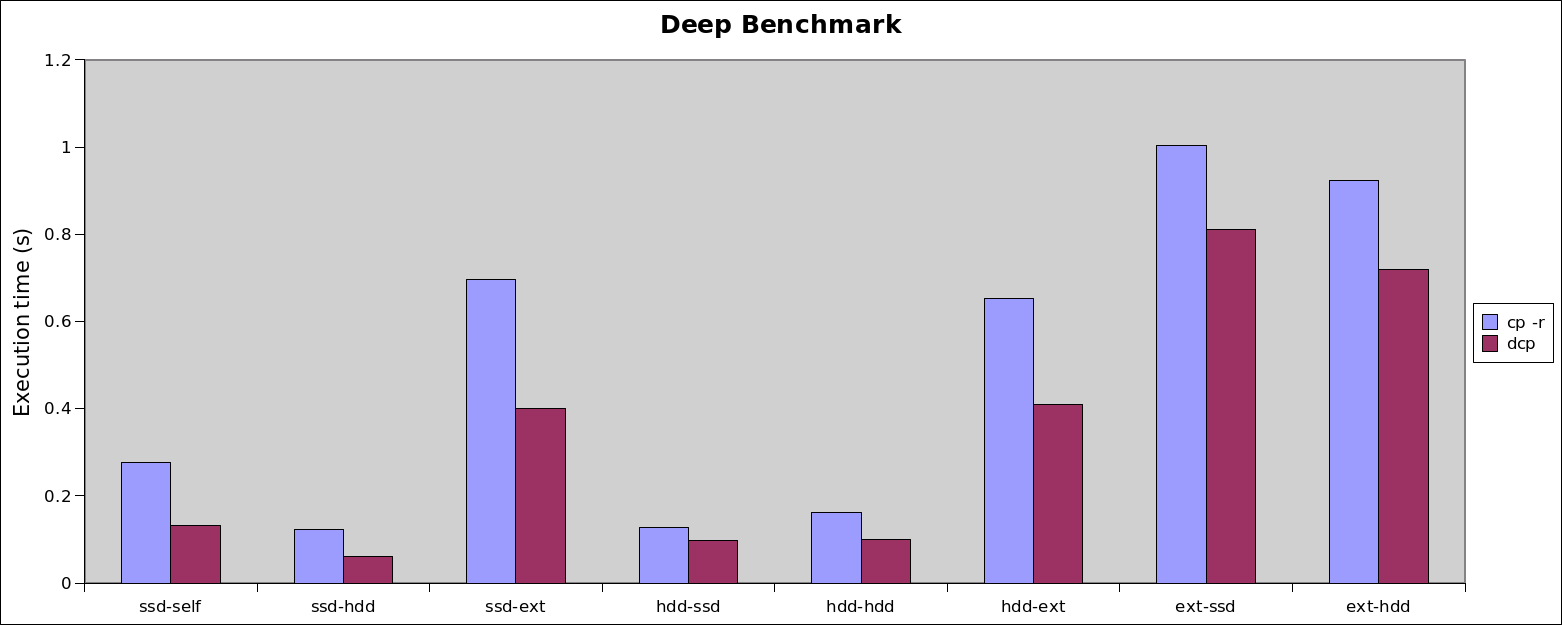
\includegraphics[width=500pt]{report/graphs/deep-manydisk.png}

\vspace{5mm}

The deep benchmark results reflect the same statistically significantly lower
execution time of dcp than 'cp -r' ($p < 0.005$). Contrasting with the previous
benchmarks, ssd-ext shows a significantly (1.7x) higher copy time for 'cp -r' than
dcp. This is perhaps indicative of the fact that raw throughput may be the limiting
factor when copying files across a USB interface, and that smart prioritization of
tasks when copying smaller amounts of data allows the kernel to intelligently
batch writes in such a way that the external drive minimizes seek time. This particular
test, due to the small volume of data copied, is aimed more at testing a potential weakness
of dcp than a practical situation. \\

Finally, the results of running the deep benchmark with certain optimizations turned off
are displayed in the following graph.\\

\vspace{5mm}

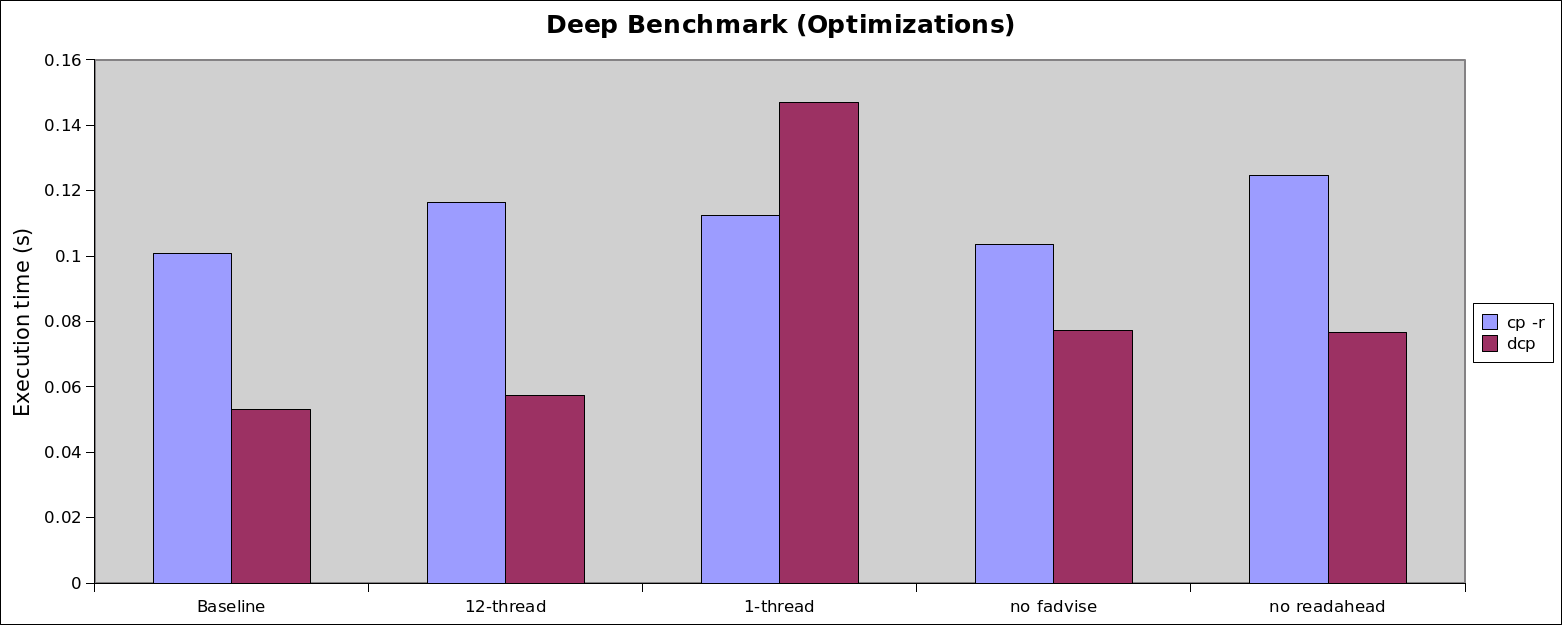
\includegraphics[width=500pt]{report/graphs/deep-optimizations.png}

\vspace{5mm}

The statistically significant optimizations for the deep benchmark included
only the 1-thread test ($p < 0.001$). However, the deep benchmark experienced
large standard deviations in each data set, ranging from 21\% to over 40\%
of the mean. This volatility contrasts with the previous fat benchmark,
where standard deviations were typically around 10\% of the mean. Thus,
it is difficult to draw conclusions from the performance of the deep benchmark,
but as mentioned earlier the deep benchmark is not an entirely realistic test
case, so it is not overly important to fully understand which optimizations
work hardest in this benchmark. \\

In all 3 selective optimization benchmarks, it is apparent that the major
factors which make dcp faster than cp -r are, as expected, multithreading,
and by extension asynchronous IO, and, to a lesser extent, fadvise and readahead.
Disabling multithreading in any of the benchmarks resulted in a large decrease
in performance for all 3 benchmarks. The other effects, including changing
the number of threads and the effects of fadvise and readahead are a bit more
difficult to describe qualitatively. For different workloads, different optimizations
are applicable, and the previous sections have attempted to explain why these
particular optimizations caused statistically significant variance in performance
for each benchmark. \\


\section{Practical test}
Additionally, one practical test was done to demonstrate the advantage
of dcp over standard cp -r. 5.7gb of video files split among 5 subdirectories were copied between
HDD A and HDD B to simulate a backup of videos, a usage pattern common for one of the researchers.
This benchmark was not repeated for other drive types as it is simply intended to convey a practical example use
case. \\

The results on this practical test show that dcp in its current state outperforms cp -r by a decent margin even
in situations where a disk's theoretical maximum throughput is approached (typically with large sequential reads/writes).
The mean execution time of cp -r is approximately 2:10, while the mean execution time of dcp is 1:50, with a sample standard deviation of
5 seconds and $p < 0.01$. Roughly calculating the raw throughput, dcp copies at approximately 53 mb/s while 'cp -r' copies
at approximately 45mb/s. It is noteworthy that the CrystalDiskBenchmark results for HDD B indicated that it has a sequential
write throughput of 55mb/s when the disk was benchmarked 2.5 years earlier (when it was new) by one of the researchers. \\

\section{Observations}
One interesting observation is that tests done on the first test platform took significantly longer
than tests done on the second test platform for similar disk configurations. While more testing and
research is necessary to ascertain the cause of this performance discrepancy, one key difference between
the platforms which may have caused this behavior is that test platform 1 used older disks which were
about 50-60\% full, as opposed to test platform 2 which used a single new mostly-empty disk. Additionally,
the solid state drive used by test platform 1 was the boot drive, whereas the disk used by platform 2
was not. Finally, the specific behavior of prefetching, buffer caching, and file IO may have been affected by differences
in the kernel version between the two platforms, as well as the fact that platform 1 runs Ubuntu while platform 2 runs Arch. \\

\begin{thebibliography}{9}
\bibitem{rejected}
    GNU
    \emph{Coreutils - rejected feature requests}.
    \url{https://www.gnu.org/software/coreutils/rejected_requests.html}
\bibitem{cppara}
    Korb, Bruce
    \emph{Another rfe: "cp" this time}.
    \url{http://lists.gnu.org/archive/html/coreutils/2012-04/msg00079.html}
\bibitem{pcopy}
    Korb, Bruce
    \emph{pcopy}.
    \url{https://github.com/brkorb/pcopy}
\bibitem{aio}
    Asynchronous IO
    \url{http://man7.org/linux/man-pages/man7/aio.7.html}
  \bibitem{fallocate}
    Fallocate
    \url{http://man7.org/linux/man-pages/man3/posix\_fallocate.3.html}
  \bibitem{fadvise}
    \url{http://linux.die.net/man/2/posix\_fadvise}
\end{thebibliography}
\end{document}
